\begin{figure}[t]
\centering
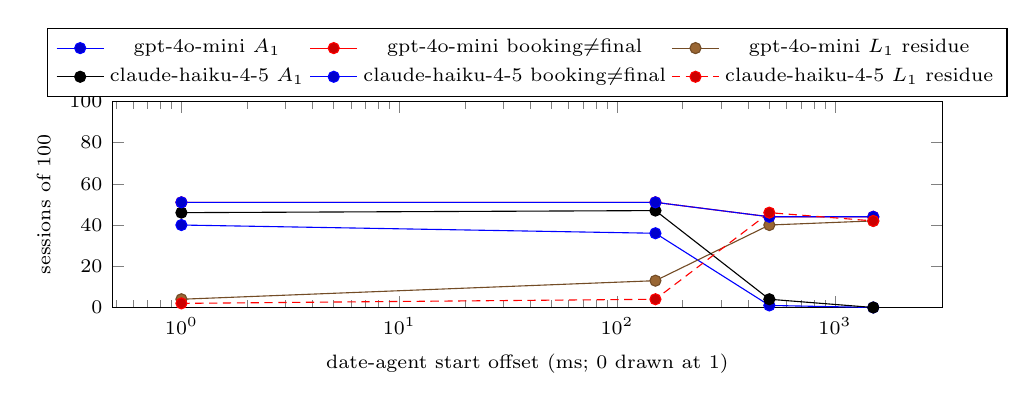
\begin{tikzpicture}
\begin{axis}[width=\columnwidth, height=4.2cm, xmode=log, log basis x=10, xlabel={date-agent start offset (ms; 0 drawn at 1)},
  ylabel={sessions of 100}, ymin=0, ymax=100, legend style={font=\scriptsize, at={(0.5,1.02)}, anchor=south, legend columns=3}, tick label style={font=\scriptsize}, label style={font=\scriptsize}]
\addplot+[mark=*] coordinates {(1,40) (150,36) (500,1) (1500,0)};
\addlegendentry{gpt-4o-mini $A_1$}
\addplot+[mark=*] coordinates {(1,51) (150,51) (500,44) (1500,44)};
\addlegendentry{gpt-4o-mini booking$\neq$final}
\addplot+[mark=*] coordinates {(1,4) (150,13) (500,40) (1500,42)};
\addlegendentry{gpt-4o-mini $L_1$ residue}
\addplot+[mark=*] coordinates {(1,46) (150,47) (500,4) (1500,0)};
\addlegendentry{claude-haiku-4-5 $A_1$}
\addplot+[mark=*] coordinates {(1,51) (150,51) (500,44) (1500,44)};
\addlegendentry{claude-haiku-4-5 booking$\neq$final}
\addplot+[mark=*] coordinates {(1,2) (150,4) (500,46) (1500,42)};
\addlegendentry{claude-haiku-4-5 $L_1$ residue}
\end{axis}
\end{tikzpicture}
\caption{Probe 303: the live \A1 rate and the outcome as a function of the date agent's start offset (revision probability $0.5$; $n=100$ per cell).}
\label{fig:offset}
\end{figure}
